\documentclass{article}

\usepackage{amsmath,amssymb}
\usepackage{tikz}
\usepackage{pgfplots}
\usepackage{xcolor}
\usepackage[left=2.1cm,right=3.1cm,bottom=3cm,footskip=0.75cm,headsep=0.5cm]{geometry}
\usepackage{enumerate}
\usepackage{enumitem}
\usepackage{marvosym}
\usepackage{tabularx}
\usepackage{multirow}

\usepackage{listings}
\definecolor{lightlightgray}{rgb}{0.95,0.95,0.95}
\definecolor{lila}{rgb}{0.8,0,0.8}
\definecolor{mygray}{rgb}{0.5,0.5,0.5}
\definecolor{mygreen}{rgb}{0,0.8,0.26}
\lstdefinestyle{java} {language=java}
\lstset{language=java,
	basicstyle=\ttfamily,
	keywordstyle=\color{lila},
	commentstyle=\color{lightgray},
	stringstyle=\color{mygreen}\ttfamily,
	backgroundcolor=\color{white},
	showstringspaces=false,
	numbers=left,
	numbersep=10pt,
	numberstyle=\color{mygray}\ttfamily,
	identifierstyle=\color{blue},
	xleftmargin=.1\textwidth, 
	%xrightmargin=.1\textwidth,
	escapechar=§,
}

\usepackage[utf8]{inputenc}
\usepackage{hyperref}
\hypersetup{
	colorlinks,
	citecolor=blue,
	filecolor=blue,
	linkcolor=blue,
	urlcolor=blue
}

\renewcommand*{\arraystretch}{1.4}

\newcolumntype{L}[1]{>{\raggedright\arraybackslash}p{#1}}
\newcolumntype{R}[1]{>{\raggedleft\arraybackslash}p{#1}}
\newcolumntype{C}[1]{>{\centering\let\newline\\\arraybackslash\hspace{0pt}}m{#1}}

\newcommand{\E}{\mathbb{E}}
\renewcommand{\epsilon}{\varepsilon}
\DeclareMathOperator{\rk}{rk}
\DeclareMathOperator{\Var}{Var}
\DeclareMathOperator{\Cov}{Cov}
\DeclareMathOperator{\Cor}{Cor}
\DeclareMathOperator{\SD}{SD}

\title{\textbf{Grundlagen des Finanzmanagements, Tutorium 6}}
\author{\textsc{Henry Haustein}}
\date{}

\begin{document}
	\maketitle
	
	\section*{Aufgabe 16.11: Ausbeutung von Fremdkapitalgebern}
	\begin{enumerate}[label=(\alph*)]
		\item Die Rendite $\frac{Kapitalwert}{\text{Investition}}$ der einzelnen Projekte ist
		\begin{itemize}
			\item Projekt A: 20 \%
			\item Projekt B: 12 \%
			\item Projekt C: 11.76 \%
			\item Projekt D: 50 \%
			\item Projekt E: 24 \%
		\end{itemize}
		Die Fremdkapitalgeber fordern folgende Mindestrendite (Formel steht in der Vorlesungsunterlagen)
		\begin{align}
			\frac{\beta_{FK}}{\beta_{EK}} \cdot \text{Verschuldungsgrad} = \frac{0.3}{2}\cdot 1.2 = 0.18 \notag
		\end{align}
		Damit werden die Projekte A, D und E durchgeführt.
		\item Die Projekte B und C werden nicht durchgeführt. Dadurch entgeht dem Unternehmen ein Gewinn von 6 + 10 = 16.
	\end{enumerate}
	
	\section*{Aufgabe 2K322: Kapitalstruktur}
	\begin{enumerate}[label=(\alph*)]
		\item Unternehmen B hat doppelt so viel Kapital wie Unternehmen A, damit sollte es auch einen doppelt so großen Bruttogewinn machen, also 220 Mio. \EUR. Die Eigenkapitalkosten sind
		\begin{align}
			110\text{ Mio. \EUR} &= 300 \text{ Mio. \EUR}\cdot 0.08 + 700\text{ Mio. \EUR}\cdot r_{EK} \notag \\
			r_{EK} &= 12.29\text{ \%}\notag \\
			220\text{ Mio. \EUR} &= 1000 \text{ Mio. \EUR}\cdot 0.08 + 1000\text{ Mio. \EUR}\cdot r_{EK} \notag \\
			r_{EK} &= 14\text{ \%}\notag
		\end{align}
		\item Wir sind in einer MM-Welt ohne Steuern, damit ist die Kapitalstruktur eines Unternehmens egal und die WACC's müssen gleich sein.
		\item Ist Arbitrage möglich? $r_{WACC,A}=0.11$ vs. $r_{WACC,C}=\frac{160\text{ Mio. \EUR}}{1.5\text{ Mrd. \EUR}}=0.1067$. Alle Aktien von C verkaufen ergibt $C=150$ Mio. \EUR. Weiteres Kapital aufnehmen/Kapital anlegen:
		\begin{align}
			NOM &= C\cdot\frac{L_{alt}-L_{neu}}{L_{neu}+1} = 150\text{ Mio. \EUR}\cdot\frac{\frac{300\text{ Mio. \EUR}}{700\text{ Mio. \EUR}}-\frac{1}{2}}{\frac{1}{2}+1}\notag \\
			&= -7.14\text{ Mio. \EUR} \notag
		\end{align}
		Dieses Geld wird also zum risikolosen Zinssatz angelegt und mit dem restlichen Geld $C+NOM=142.86\text{ Mio. \EUR}$ werden Aktien von A gekauft. Der Arbitragegewinn ist damit
		\begin{align}
			\text{Arbitragegewinn} &= \frac{C+NOM}{EK_{neu}}\cdot\text{Nettogewinn}_{neu} - NOM\cdot r_f - w\cdot\text{Nettogewinn}_{alt} \notag \\
			&= 22.45\text{ Mio. \EUR} + 0.57\text{ Mio. \EUR} - 16\text{ Mio. \EUR} \notag \\
			&= 7.02\text{ Mio. \EUR} \notag
		\end{align}
		Der individuelle Zinssatz beträgt
		\begin{align}
			r_i = \frac{\frac{C+NOM}{EK_{neu}}\cdot\text{Nettogewinn}_{neu} - NOM\cdot r_f}{C} = 15.35\text{ \%} \notag
		\end{align}
		Der Barwert des Arbitragegewinns ist also $\frac{7.02\text{ Mio. \EUR}}{0.1535}=45.73\text{ Mio. \EUR}$.
		\item Es gilt $r_{GK}=r_{EK}\cdot\frac{EK}{GK} + r_{FK}\cdot\frac{FK}{GK}\to\min$
		\begin{itemize}
			\item Verschuldungsgrad 0: $r_{GK}=11\text{ \%}\cdot \frac{1}{1} + 0\text{ \%}\cdot\frac{0}{1}=11\text{ \%}$
			\item Verschuldungsgrad 0.5: $r_{GK}=12.5\text{ \%}\cdot \frac{2}{3} + 7\text{ \%}\cdot\frac{1}{3}=10.67\text{ \%}$
			\item Verschuldungsgrad 1: $r_{GK}=13.5\text{ \%}\cdot \frac{1}{2} + 7.5\text{ \%}\cdot\frac{1}{2}=10.5\text{ \%}$
			\item Verschuldungsgrad 2: $r_{GK}=14\text{ \%}\cdot \frac{1}{3} + 8\text{ \%}\cdot\frac{2}{3}=10\text{ \%}$
			\item Verschuldungsgrad 3: $r_{GK}=15\text{ \%}\cdot \frac{1}{4} + 8.5\text{ \%}\cdot\frac{3}{4}=10.125\text{ \%}$
			\item Verschuldungsgrad 4: $r_{GK}=16\text{ \%}\cdot \frac{1}{5} + 9\text{ \%}\cdot\frac{4}{5}=10.4\text{ \%}$
		\end{itemize}
		Offenbar ist Verschuldungsgrad 2 optimal. Das heißt die 1 Mrd. \EUR\, müssen in 333 Mio. \EUR\, EK und 667 Mio. \EUR\, FK aufgeteilt werden. Aktuell besitzt das Unternehmen 700 Mio. \EUR\, EK, es muss also 367 Mio. \EUR\, EK in FK umwandeln. \\
		Wir befinden uns hier nicht mehr in einer MM-Welt, weil die FK-Zinsen steigen wegen des Insolvenzrisikos (statt konstant zu bleiben) und damit auch $r_{GK}$ steigt anstatt konstant zu bleiben.
		\item Eine Steigerung des Unternehmenswertes ist nur durch das Tax Shield möglich, also $\Delta V=s\cdot\Delta D$, damit $70\text{ Mio. \EUR}=0.35\cdot\Delta D \Rightarrow \Delta D=200\text{ Mio. \EUR}$.
		\item z.B. Insolvenzkosten für den Insolvenzverwalter, aber auch der Verlust von Kunden und Lieferanten und für FK-Geber die eventuell nicht mehr zurückgezahlten Zinsen.
	\end{enumerate}

	\section*{Aufgabe 3K311: Kapitalstrukturtheorie}
	\begin{enumerate}[label=(\alph*)]
		\item MM1: $V_L=V_U+s\cdot D$ \\
		MM2: $r_{EK}=r_U + L\cdot (1-s)\cdot (r_U-r_D)$
		\item Es muss ein vollkommener Kapitalmarkt vorliegen, das heißt unter anderem
		\begin{itemize}
			\item keine Steuern auf Transaktionen: Scheint es aktuell nicht zu geben, aber Olaf Scholz plant welche.
			\item keine Transaktionskosten: Je nach Broker müssen Spesen und Provisionen bezahlt werden.
			\item keine Emissionskosten: Eine Emission an einer Börse kostet Geld.
			\item keine Informationsasymmetrien: (professionelle) Investoren wissen in der Regel schon sehr gut, wie es dem Unternehmen geht.
			\item kein Insolvenzrisiko: Es gibt definitiv ein Insolvenzrisiko.
			\item Sollzins = Habenzins: Habenzinsen sind aktuell bei 0 \%, aber Sollzinsen bei etwa 2 \%.
			\item Jeder kann sich Geld zu gleichen Konditionen borgen: Bonität einer Person spielt eine Rolle.
			\item Marktteilnehmer haben homogene und rationale Erwartungen über die Cashflows eines Unternehmens: Bewertungen von Analysten gehen weit auseinander.
		\end{itemize}
		\item Graphen:
		\begin{center}
			\begin{tikzpicture}
				\begin{axis}[
					xmin=0, xmax=1, xlabel=$L$,
					ymin=0, ymax=1, ylabel=$r_i$,
					title={MM ohne Steuern},
					samples=400,
					axis x line=middle,
					axis y line=middle,
					domain=0:1,
					yticklabels={,,},
					xticklabels={,,},
					xtick style={draw=none},
					ytick style={draw=none},
					]
					\addplot[mark=none,smooth,blue] {0.2};
					\addplot[mark=none,smooth,red] {0.5+0.5*x};
					\addplot[mark=none,smooth,green!80!black] {0.5};
					
				\end{axis}
			\end{tikzpicture}
			\begin{tikzpicture}
				\begin{axis}[
					xmin=0, xmax=1, xlabel=$L$,
					ymin=0, ymax=1, ylabel=$r_i$,
					title={MM mit Steuern},
					samples=400,
					axis x line=middle,
					axis y line=middle,
					domain=0:1,
					yticklabels={,,},
					xticklabels={,,},
					xtick style={draw=none},
					ytick style={draw=none},
					]
					\addplot[mark=none,smooth,blue] {0.1};
					\addplot[mark=none,smooth,red] {0.5+0.5*x};
					\addplot[mark=none,smooth,green!80!black] {0.5-0.4*x};
					
				\end{axis}
			\end{tikzpicture}
			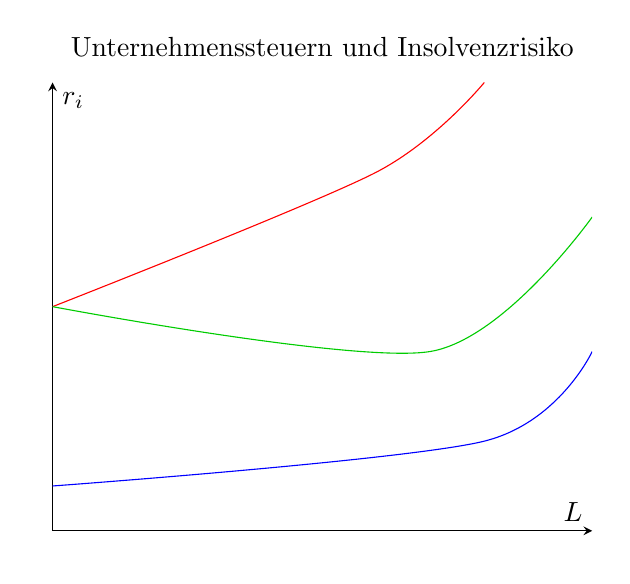
\begin{tikzpicture}
				\begin{axis}[
					xmin=0, xmax=1, xlabel=$L$,
					ymin=0, ymax=1, ylabel=$r_i$,
					title={Unternehmenssteuern und Insolvenzrisiko},
					samples=400,
					axis x line=middle,
					axis y line=middle,
					domain=0:1,
					yticklabels={,,},
					xticklabels={,,},
					xtick style={draw=none},
					ytick style={draw=none},
					]
					\addplot[blue,smooth] coordinates {
						(0,0.1)
						(0.8,0.2)
						(1,0.4)
					};
					\addplot[red,smooth] coordinates {
						(0,0.5)
						(0.6,0.8)
						(0.8,1)
					};
					\addplot[green!80!black,smooth] coordinates {
						(0,0.5)
						(0.7,0.4)
						(1,0.7)
					};
					
				\end{axis}
			\end{tikzpicture} \\
			\textcolor{blue}{FK}, \textcolor{red}{EK}, \textcolor{green!80!black}{GK}
		\end{center}
		\item In einer MM-Welt ohne Steuern ist die Kapitalstruktur egal; in einer MM-Welt mit Steuern sollte durch das Tax Shield so viel FK wie nur möglich im Unternehmen sein und bei Insolvenzrisiko gibt es eine optimale Verschuldung.
		\item Verkauf der Aktien der Lever AG bringt $C=w\cdot 10\text{ Mio. \EUR}$. Kreditaufnahme:
		\begin{align}
			NOM &= C\cdot\frac{L_{alt}-L_{neu}}{L_{neu}+1} = w\cdot 10\text{ Mio. \EUR}\cdot\frac{1-0}{0+1}\notag \\
			&= w\cdot 10\text{ Mio. \EUR} \notag
		\end{align}
		Davon werden die Aktien der Nodebt AG gekauft und der Arbitragegewinn ist
		\begin{align}
			\text{Arbitragegewinn} &= \frac{C+NOM}{EK_{neu}}\cdot\text{Nettogewinn}_{neu} - NOM\cdot r_f - w\cdot\text{Nettogewinn}_{alt} \notag \\
			&= \frac{w\cdot 20\text{ Mio. \EUR}}{19.8\text{ Mio. \EUR}}\cdot 2.2\text{ Mio. \EUR} - w\cdot 10\text{ Mio. \EUR}\cdot 0.1 - w\cdot (2.2\text{ Mio. \EUR} - 0.1\cdot 10\text{ Mio. \EUR}) \notag \\
			&= w\cdot 2.22\text{ Mio. \EUR} - w\cdot 1\text{ Mio. \EUR} - w\cdot 1.2\text{ Mio. \EUR} \notag \\
			&= w\cdot 0.02\text{ Mio. \EUR} \notag
		\end{align}
		Der individuelle Zinssatz beträgt
		\begin{align}
			r_i = \frac{\frac{C+NOM}{EK_{neu}}\cdot\text{Nettogewinn}_{neu} - NOM\cdot r_f}{C} = \frac{w\cdot 2.22\text{ Mio. \EUR} - w\cdot 1\text{ Mio. \EUR}}{w\cdot 10\text{ Mio. \EUR}} = 12.2\text{ \%} \notag
		\end{align}
		Damit gilt
		\begin{align}
			BW = \frac{w\cdot 0.02\text{ Mio. \EUR}}{0.122} = w\cdot 0.164\text{ Mio. \EUR} &\overset{!}{=} 0.121\text{ Mio. \EUR} \notag \\
			w &= 73.78\text{ \%} \notag
		\end{align}
	\end{enumerate}
	
\end{document}